\section{Approach} \label{sec:approach}

The two proposed genotype-phenotype map learning techniques are based on artificial neural network autoencoders.
These are networks that are trained to regurgitate as output the input that they were provided.
Such networks are used to discover efficient lower-dimensional codings for datasets and, more recently, as method for generative modeling \cite{liou2014autoencoder, kingma2013auto}.

\begin{figure}
  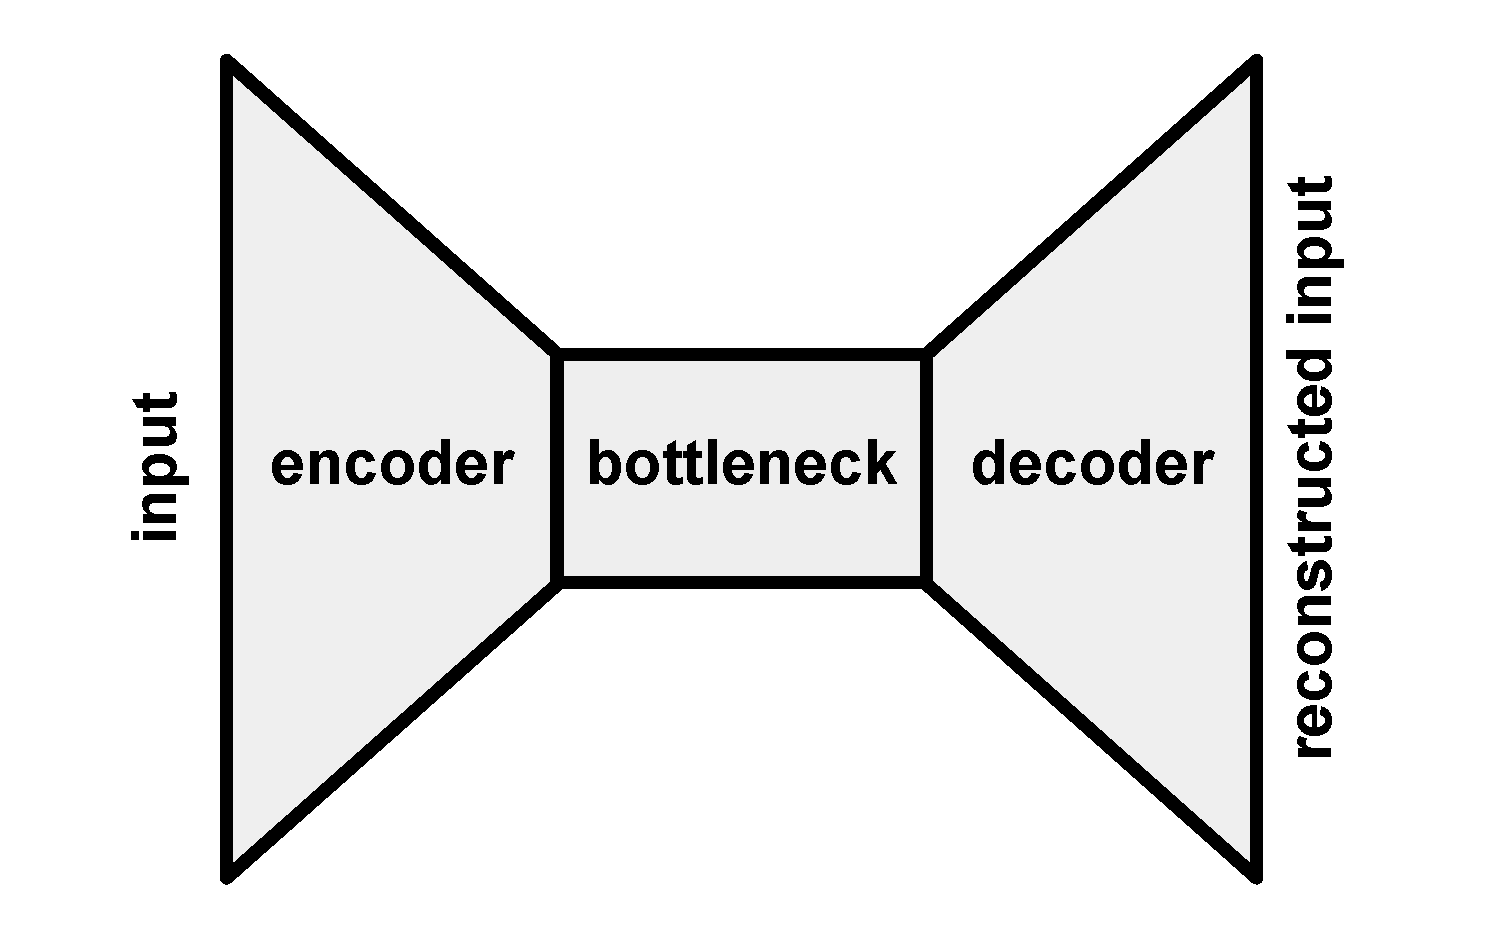
\includegraphics[width=0.5\linewidth]{img/bottleneck}
  \caption{Schematic of a bottlenecked autoencoder.}
  \label{fig:bottleneck}
\end{figure}


The first technique uses a bottlenecked autoencoder.
Figure \ref{fig:bottleneck} provides a schematic impression of such an autoencoder.
This autoencoder has a small layer in the middle that information must pass through to reach the output.
Thus, the autoencoder is forced to learn a compact representation for the input it is trained with that can pass through the bottleneck.
The part of the autoencoder that precedes the bottleneck is called the encoder and the part that follows is called the decoder.
This autoencoder will be trained to encode phenotypes taken from fitness peaks throughout an evolutionary search space.
The idea of this approach is that, because the bottleneck provides a compact representation of those high-fitness phenotypes, using the decoder as a genotype-phenotype mapping will readily allow mutation to move the phenotype between otherwise distant fitness peaks.

\begin{figure}
  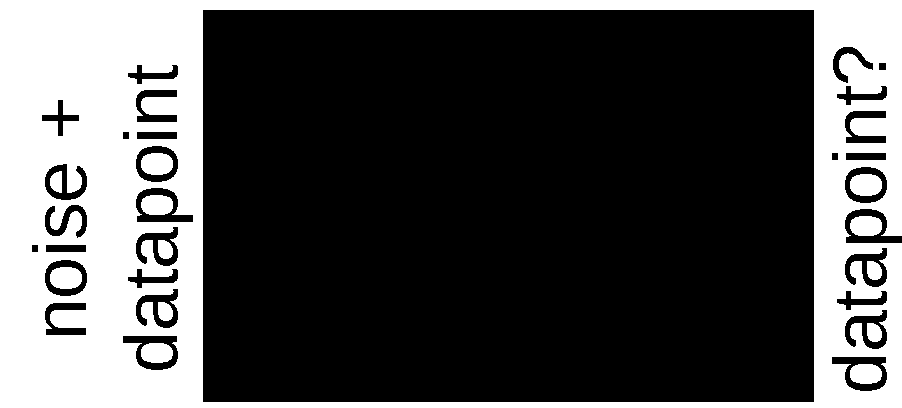
\includegraphics[width=\linewidth]{img/denoiser}
  \caption{
    Schematic of a denoising autoencoder.
  }\label{fig:denoiser}
\end{figure}


The second technique uses a denoising autoencoder.
Figure \ref{fig:denoiser} provides a schematic depiction of such an autoencoder.
These autoencoders have not bottleneck.
Instead, they are trained to reconstruct noisy input into its original unadulterated form.
This autoencoder will be trained to reconstruct phenotypes taken from fitness peaks throughout an evolutionary search space.
For this approach, the entire denoising autoencoder would be used as the genotype-phenotype mapping.
The idea of this design is that mutations that would otherwise be deleterious will effectively be interpreted as noise and prevented from being expressed by the genotype-phenotype mapping.
Effectively, this mapping should flatten out the valleys between local fitness peaks to allow evolution to more readily drift between those local fitness peaks.
